\documentclass[UKenglish]{ifimaster}

\usepackage{thesisstyle}

\addbibresource{references.bib}
\addbibresource{proceedings.bib}

\title{Automated Assessment of Norwegian L2 Essays}
\subtitle{Using Multi-task Learning}
\author{Stig Johan Berggren}

\renewcommand*\rmdefault{ptm}

\begin{document}
\duoforside[
  dept={Department of Informatics},
  program={Language and Communication},
  short
]

\frontmatter{}

% \chapter*{Abstract}

% \tableofcontents{}
% \listoffigures{}
% \listoftables{}

% \chapter*{Preface}

\mainmatter{}

\chapter{Background}

\section{Background}

In this essay, I cover some of the background concerning the Native Language
Identification and Automated assessment tasks, which are well studied in the
field of natural language processing (NLP). I will examine how these tasks
may be addressed simultaneously using multi-task learning and some approaches
to the separate tasks that have been found useful in previous work. The topic
of multi-task learning will also be discussed in the essay.

The first section covers background related to machine learning and different
neural methods. Then, we will look at the properties of learner language, and
the specific tasks of automated scoring and native language identification.
We will also look at a selection of datasets of learner language that have
been used for these tasks previously.


\section{Tasks and machine learning}

Machine learning (ML) is a field that covers a wide range of different
techniques and algorithms for ``teaching'' computers to perform well at a
range of tasks. Examples of tasks may be categorizing a document or detecting
an object in an image. Techniques in machine learning are often categorized
under labels such as \emph{supervised learning}, \emph{unsupervised
learning}, and \emph{reinforcement learning}.

The first two are applicable when we have training data available. Supervised
learning utilizes a set of training examples with target labels in order to
train a model that predict true labels for new, unseen data. In the essay
scoring task discussed below, for instance, training data consists of essays
that already have assigned a grade, and the resulting, trained model should
be able to assign a ``correct'' grade to any essay, including those it has
never seen during training.

Unsupervised learning is a range of techniques which do not use target labels
in training, but are still able to ``learn'' useful representations and
groupings of the training data. Unsupervised learning can be part of a more
complex model, for instance when using embeddings as feature representations
in a neural network. Embeddings map sparse features (e.g. words/tokens) to a
dense, low-dimensional space, using contexts to discover what tokens are
similar and should exist close to each other in this \emph{embedding space}.

Many machine learning algorithms are based on statistical modelling and
concepts from linear algebra, with low-level routines such as matrix
multiplication being central to the algorithms.

In the field of natural language processing, algorithms in the neural network
family are gaining ground on the more ``traditional models'' in the field,
which have generally been linear models such as support vector machines and
logistic regression \autocite[345]{goldberg2016primer}. Compared to the
traditional models, neural networks often require less focus on feature
design and hand-crafting features. On the other hand, feature representations
such as word embeddings are important.


\subsection{Neural networks}

Neural networks is a family of machine learning models. These models are
based upon units often referred to as ``neurons'', which are capable of
computing a weighted sum of inputs and applying a non-linear \emph{activation
function} to the result. The networks are usually trained with supervised
learning, where the performance on training samples is measured using an
\emph{objective} function or \emph{loss} function, which is minimized by
backpropagation. In order for backpropagation to work, it is crucial that the
activation function is differentiable.

One of the simplest models in the neural networks family is the perceptron.
It is only capable of calculating a weighted sum across a feature vector and
applying a threshold function. This threshold function is not differentiable,
and the perceptron is therefore not trained with backpropagation.
Historically, one of the most used activation functions is the sigmoid
function: \(s(x) = {(1 + e^{-x})^{-1}}\). Nowadays, one of the most common
activations is the rectified linear unit (ReLU): \(f(x) = \max(x, 0)\). ReLU
is, strictly speaking, not differentiable, because of its hinge at $x = 0$.
Regardless it works well in practice, since almost all pre-activation values
will be different from zero. The zero case can be treated as a special case,
to avoid undefined values.

\subsubsection{Multi-layer perceptron}

\begin{figure}
  \centering
  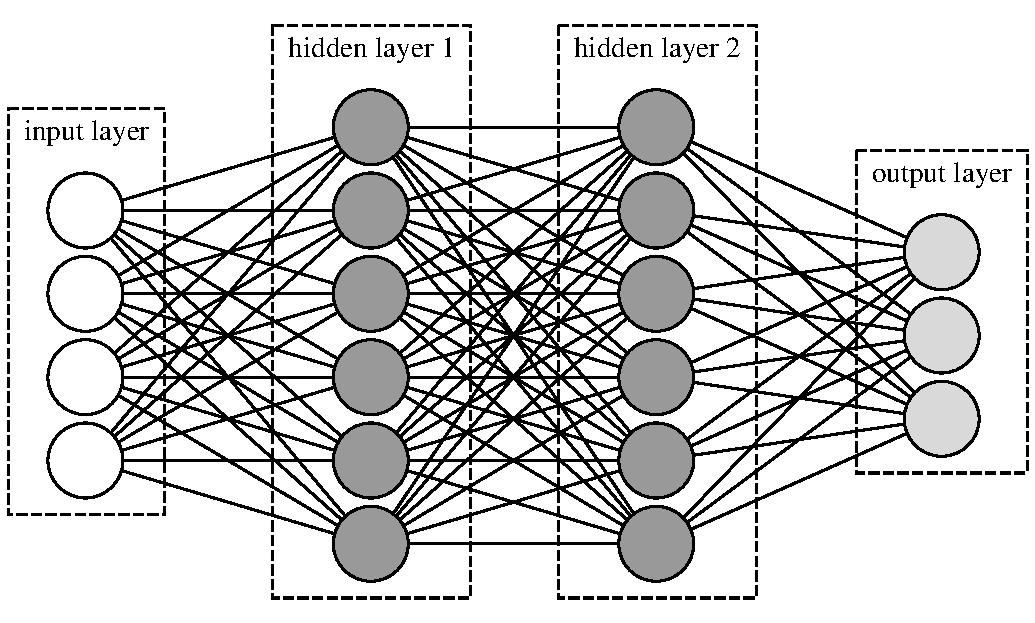
\includegraphics[width=0.8\textwidth]{graph}
  \caption{A fully connected feed-forward neural network with four input
  nodes, two hidden layers, and three output nodes.}
  \label{mlp-diagram}
\end{figure}

The ``vanilla'' neural network is the feed-forward network, also known as the
\emph{multi-layer perceptron} (MLP). This model incorporates one or more
hidden layer in-between the input layer (the feature vector) and the output
layer. A diagram of an example MLP with two hidden layers can be seen in
figure \ref{mlp-diagram}. For multi-class prediction, the output layer
typically uses a \emph{softmax} activation. This has the property of
restricting each output value to be in the interval $(0,1)$, and additionally
makes sure all output values sum to $1$. These properties allow the outputted
values to be interpreted as a probability distribution.


\subsubsection{Convolutional neural networks}

Convolutional neural networks (CNN) can exploit local patterns in the input,
unlike the MLP, which has no way to identify elements of the input layer as
being ``close'' to each other in any sort of measure. CNNs use convolutional
layers to make these local relationships explicit.

CNNs are widely employed in image processing models, using
two-di\-men\-sional convolutional layers. These models can often get very
deep, using a number of convolutional layers at different levels in the
network, interspersed with pooling or downsampling layers.

There are also NLP applications where CNNs can be employed. Unlike images,
data in NLP is usually sequential or one-dimensional, but it may be converted
into two dimensions, for example by replacing each word by an embedding
vector.


\subsubsection{Recurrent neural networks}

Recurrent networks (RNN) are suited to sequential data. They make have an
internal \emph{state} that is passed between time steps. A benefit of RNNs is
that they can accept input of any length and also produce sequential output
of any length. This in contrast to feed-forward neural networks, which take a
fixed-length vector as their input.

A long standing problem in training RNNs was that when applying
backpropagation through time, the gradient values can tend toward zero or
diverge because of multiplication across many time steps. This is known as
the \emph{vanishing} and \emph{exploding gradients problem}, respectively.
Mitigation techniques include replacing the units of the network with what's
known as \emph{gated units}, that are especially designed to address these
problems. Gated recurrent units (GRU) and Long short-term memory (LSTM) are
widely used gated units in RNNs.


\subsubsection{Natural language features}

For applications of machine learning in NLP, we often want to use the words
in a document as features. However, the vast number of different words in a
language can lead to inefficient use of memory and computing power if the
words are represented naively, for instance with a one-hot vector encoding
with the vector having the number of dimensions equal to the size of the
lexicon. It is therefore useful to map words to a lower-dimensional
representation, known as an \emph{embedding}.

\sloppy Training embeddings rely on the distributional hypothesis, namely
that words with similar meanings are likely to appear in similar contexts.
Therefore, without prior knowledge of any words in a language, the resulting
embeddings are likely to put words with similar meanings close to each other
in the embedding space. It has also been observed that semantic relations
between words, for instance regarding gender or inflection, corresponds to
defined directions in the embedding space\autocite{mikolov2013linguistic}.
These relations can be found by subtracting word vectors. A famous example of
an emergent analogy learned by the embeddings is: ``Man is to king as woman
is to ...''. In terms of arithmetic on embedding vectors, the embeddings
modelled the analogy as $\vec{king}-\vec{man}+\vec{woman}\approx\vec{queen}$.
\fussy

There exists a number of embedding models, including Word2Vec
\autocite{mikolov2013word2vec} and GloVe \autocite{pennington2014glove}.
These models can be used to compute embeddings based on new training data, or
one may use pre-trained embeddings.

Different approaches to embeddings may be necessary for different languages.
A word-based approach can work well for a relatively analytic language such
as English, but be less suited for agglutinative or synthetic languages,
because of the differing amount of semantic information present in a single
token. A converse problem occurs where a sequence of words is best analyzed
as a single unit.

Another issue is ambiguity, as the process of training embeddings only
considers the form of a word. Homographs like \emph{well}, which can be both
an adverb adn a noun, are each mapped to a single embedding vector, with no
way to distinguish the different meanings of the word.

It is also possible to embed $n$-grams of characters instead of words. A
disadvantage of this approach is that it becomes more difficult to
distinguish words with similar spelling, but different meaning, and it does
not solve the problem of homographs. However, it seems that the embeddings
may still be more robust when encountering spelling mistakes. The embeddings
based on word forms will see ``beautiful'' and ``beutiful'' as completely
separate words, while there still exists similarities between them on the
level of characters: they share a good portion of their $n$-grams. Another
advantage might be the possibility of accessing semantic meaning at a
sub-word level, including prefixes and suffixes.

For representing a document non-sequentially, a common approach is to use
continuous bag-of-words (CBOW). This is the sum or average of embedding
vectors for all active features \autocite[352]{goldberg2016primer}. CBOW thus
disregards some information, including order and whether features occur close
to each other in the document.


\subsection{Multi-task learning}

Multi-task learning refers to optimizing a target function for two or more
different tasks simultaneously \autocite{ruder17overview}. One benefit of
this approach is increased generalization. Intuitively, this is feasible
because the neural network needs to find a representation which is useful for
all the tasks it is optimizing on, and thus is less likely to pick up noise
in the data than it might be when only considering a single task. A
representation that is useful to different tasks is more likely to be able to
generalize, not only to data beyond the training data, but to new tasks which
were not part of the training process as well.

In practice, for neural networks, the tasks in question share some of the
inner layers of the network, but have separate output layers. This is called
parameter sharing. Another approach is to keep different parameters for each
of the tasks, but add a regularization loss that prevents the parameters from
diverging too much from each other. The output layers are not necessarily at
the same depth. A low-level auxiliary task can have its output layer rather
early while the main task uses more hidden layers. In the backwards pass,
losses at all the output layers should be minimized.

\textcite{ruder17} lists several tasks in natural language processing that
have been subject of experiments with multi-task learning, including machine
translation, speech recognition, semantic parsing and chunking. These tasks
have been jointly trained with auxiliary tasks such as predicting the next
word, recognizing phonemes, part-of-speech tagging, and more. Among others,
the author cites \textcite{pappas17}, who used multi-task learning to train a
document classifier using 8 different languages, sharing parameters between
the models for different languages. The model they used for this was a
hierarchical attention network.

\textcite{alonso17} investigated the effect of different auxiliary tasks and
combinations of these on a LSTM (Long Short-Term Memory) recurrent network
for sequence labelling tasks. The main tasks they considered in the study
were labelling semantic frames, semantic supersenses, named entity
recognition, ontological types for senses and Multi-Perspective Question
Answering.

They used an auxiliary task called \textsc{FreqBin}, whose objective is to
predict the log frequency of a word, discretized into a number of bins. This
study tried a new binning strategy which improved the utility of
\textsc{FreqBin} as an auxiliary task compared with previously examined
strategies. While the previous variants took the logarithm of the token's
frequency in a chosen base and rounded down to the nearest integer, the new
strategy ranked all tokens by frequency grouped them into labels by a given
quantile. In the study, they used $k=5$, yielding 5 \textsc{FreqBin} labels
with the same number of examples each.


\section{Learner language}

In the linguistic field of second language acquisition (SLA), linguists have
described characteristics of the language of people who are learning a second
language. It is common to refer to a person's first language(s), that is the
language(s) they learned when they first started to speak, as L1, and any
languages acquired later in life as L2. Since language acquisition is a
gradual process, we can speak of an \emph{interlanguage}, which is an
idiolect with systematic rules belonging to the learner in question, but
which is different from their target language. Interlanguage is not stable,
but changes as part of a learner's acquisition process
\autocite[358]{myers-scotton}.

Interlanguage can show influences from the learner's L1 in several respects,
for instance intonation and produced phonemes in pronunciation, syntactic
mistakes like inflection and word order, or even the literal translation of
idioms that do not exist in the same form in the target language. The study
of linguistic \emph{transfer} is an attempt to understand these influences.


\subsection{Automated assessment}

Assessment of proficiency, or automatic essay scoring (AES), has been framed
as a supervised learning task, using a corpus of learner texts that have each
been labelled with a proficiency rating. Automating the assessment task can
benefit applications in language education. People learning a new second
language will benefit from feedback as to which proficiency level they might
be on, for instance in relation to the Common European Framework of Reference
for Languages (the European Framework or CEFR). This may help people who want
to take language examination to find the appropriate timing and level of
testing, since an examination can be both an economical and logistical
inconvenience. Automation also allows students to receive feedback quicker
and more frequently.

Previous work by \textcite{vajjala17} uses the TOEFL11 corpus of non-native
English \autocite{blanchard13} and the First Certificate of English (FCE)
corpus \autocite{yannakoudakis2011new}. This study examines which features
may be most informative in relation to the task, and whether these are the
same features for different datasets. \citeauthor{vajjala17} uses a number of
linguistic features for the task, including several different measures for
the lexical diversity, distribution of part-of-speech (POS) tags, and
syntactic complexity. The models in the study utilize up to 116 different
features. Applied pre-processing includes syntactic parsing of sentences in
order to extract features from the parse trees. These syntactic features
include measures of average sentence length, clauses per sentence, the height
of the parse tree etc. Several of these features were based on previous work
on measuring syntactic complexity in L2 writing by
\textcite{lu2010automatic}.

Other features are designed to capture discourse properties of the text,
based on reference chains. The English language has different ways of
referring to previous information in a discourse, which is a core element of
fluent language use. For instance, the definite/indefinite distinction is a
way to reference previous information in English. This is not the case
cross-linguistically, so features like this are language-specific.
\citeauthor{vajjala17}'s features are measures of the proportions of
different pronoun types, determiners and definite noun phrases, and more, in
a reference chain, along with the average length of a reference chain.

Notably, the author did not use word or POS $n$-grams as features in the
study. The reasons given for this is that the sparse nature of $n$-gram
features make them hard to interpret, and they can introduce topic bias to
the model. The essays are written on different topics, making it likely that
certain words indicate the topic of an essay. $n$-grams can model errors
relative to the learner's target language, but she already uses features
designed to model this. Nor are character $n$-grams used as features here,
though they are generally widely used in a various NLP applications.
\citeauthor{vajjala17} also experimented with using the writing prompt and
the native language (L1) of the text's author as features.

The author trained a number of different models using different subsets of
the features. All models are linear classifiers trained with the Sequential
Minimal Optimization algorithm, a variant of support vector machines. The
model that achieved highest accuracy in the study was one that incorporated
all the features, yielding an accuracy of 73.2~\% on TOEFL11. Removing the
prompt and L1 as features resulted in a tiny drop in accuracy down to
73.0~\%.

The length of the text turned out to be one of the most informative features
in both the datasets used. However, text length correlated positively with
proficiency on TOEFL11, but negatively on the FCE corpus.


\subsection{Native Language Identification}

Native Language Identification (NLI) is the task of predicting the native
language of an author based on a text written in one of the author's second
languages (L2). The task is dependent on systematic differences between
interlanguages for learners with the same target language, but different L1s.
The feasibility of this task proves intrinsically that these systematic
differences exist, as linguists studying transfer try to explain.


\subsubsection{Shared tasks in NLI}

NLI has been the subject of three shared tasks, in 2013
\autocite{tetreault2013report}, 2016 \autocite{schuller2016interspeech} and
2017 \autocite{nli17}. The 2013 shared task used only written documents,
whereas the 2016 shared task was audio data only. Lastly, the latest shared
task in 2017 contained both written and spoken documents. Teams participating
in 2017 could choose between three tracks corresponding to written data only,
spoken data only, or both. Only teams participating in the first track, using
written data only, are considered below.

The written documents in the task was English L2 essays, written by learners
with 11 different L1s. The best-performing system in the track using only
written essays had a macro-averaged F1 score of 0.8818, using stacked
classifiers combining logistic regression on sentences with a support vector
machine (SVM) meta-classifier \autocite{cimino17}.

The best performing team which used neural networks was \textcite{li17}, who
used a multi-layer perceptron meta-classifier to combine outputs from SVM
base classifiers, and reported a F1 score of 0.8654. Another team
experimented with different neural network architectures, including RNNs and
a CNN variant known as a deep residual network \autocite{bjerva2017neural}.
Their best result was with a stacked model, combining their different models
with an SVM meta-classifier. Their best ensemble model achieved a F1 score of
0.8323, and used no external resources, i.e. no pre-trained embeddings.


\subsubsection{NLI for Norwegian}

While the shared tasks have been English learner language only, there exists
studies using different corpora with other target languages, among them
Norwegian. Norwegian NLI has been attempted by \textcite{malmasi15}, using
the ASK corpus \autocite{tenfjord06}. In their methodology, they create
artificial documents to train on by segmenting the learner texts into
sentences, then putting all the sentences from learners with the same L1 into
a bag and sampling sentences from the bag to create the new documents. Their
rationale for the methodology is that all the resulting documents are of
similar length, and that they eliminate the variation between individual
writers that otherwise might present a stronger signal than the writer's L1
alone.

In a later study \autocite{malmasi17}, they perform an NLI experiment on
several corpora, namely TOEFL11, the Norwegian ASK corpus and the Jinan
Chinese Learner corpus. However, they were not able to utilize the same
features for all the different corpora. For Norwegian, they only use the
features \emph{function word unigrams}, \emph{function word bigrams} and
\emph{part-of-speech $n$-grams}. For the English corpus, they were able to
use other features such as dependencies and context free grammar-rules. By
combining a selection of base classifiers using a Linear Discriminant
Analysis (LDA) meta-classifier trained with bootstrap aggregation (bagging),
they achieve an accuracy of $0.818$ on the Norwegian corpus.

They reapply the above methodology of generating artificial essays for the
Norwegian and Chinese corpora. In particular, they mention that this removes
bias stemming from different topics. In the case of the TOEFL11 corpus,
however, the authors of the corpus have made an effort to make the documents
balanced in terms of both L1 and the writing prompt which the learner has
answered.

Adopting this methodology, however, does mean letting go of the discourse
properties of a text, which could offer valuable cues both toward the L1, and
in relation to the automated assessment task. Moreover, it does not reflect
realistic real-world documents, which in many cases are written by
individuals, and contain bias toward specific topics.


\subsection{Datasets}

Several available datasets for different languages have been or can be used
in the tasks discussed above. Desirable properties for these tasks include
representing a broad selection of different language backgrounds and
proficiencies, a balanced selection with respect to variables such as L1 and
topic, and rich metadata. Below we will look at two corpora with English and
one with Norwegian learner texts. There exists learner corpora for several
other target languages as well, including Chinese and Czech.


\subsubsection{TOEFL11}

The TOEFL11 corpus was presented in 2013 and was specifically designed to be
suitable for the NLI task \autocite{blanchard13}. The documents are essays
from the English proficiency test TOEFL, which many take as preparation for
admission to higher education in English-speaking countries. The corpus
contains metadata for the writers' L1s and the proficiency level their essay
was assessed to. The proficiency levels are specific for the corpus and
correspond to low, medium and high proficiency, without reference to external
frameworks such as CEFR. The represented language backgrounds are Arabic,
Chinese, French, German, Hindi, Italian, Japanese, Korean, Spanish, Telugu,
and Turkish. The datasets for the NLI shared tasks in 2013 and 2017 (the
written essays) were extracted from TOEFL11.

The corpus contains 1100 essays per L1, in total 12,100 essays. The average
word count for the essays is 348, so in total the corpus contains more than
4,210,000 words.


\subsubsection{FCE}

This corpus was first introduced by \textcite{yannakoudakis2011new}. It is a
subset of the Cambridge Learner Corpus, containing the documents that were
collected from the First Certificate of English test. It contains 1238
documents, each containing a written response to two different tasks. The
documents are marked on a proficiency scale from 1 to 40.


\section{Conclusion}

The thesis will be focused on training an automated essay scoring model on
Norwegian data using multi-task learning. Native language identification is
one of possibly more auxiliary tasks that will be attepted.


\chapter{Creating a data split}

\chapter{The ASK corpus}

In this chapter we will describe the data set used throughout the thesis. The
process used to select the split between training, testing and validation
data is also described.


\section{Data set}

% cspell:disable
The ASK corpus (\emph{andrespråkskorpus}) was presented in 2006
\autocite{tenfjord06}. The corpus contains Norwegian learner essays from two
different language tests: \emph{Språkprøven i norsk for voksne innvandrere}
and \emph{Test i norsk – høyere nivå}, which test proficiency at the B1 and
B2 levels, respectively. Following the naming in
\textcite{carlsen2012proficiency}, we will refer to these tests as the
\emph{IL test} (Intermediate Level, ``Språkprøven'') and the \emph{AL test}
(Advanced Level, ``Høyere nivå'').
% cspell:enable

\begin{table}
  \centering
  \begin{tabular}{lrrr}
    \toprule
    First language             & IL test & AL test & Total \\
    \midrule
    English                    &     100 &     100 &   200 \\
    Polish                     &     100 &     100 &   200 \\
    Russian                    &     100 &     100 &   200 \\
    Somali                     &     100 &       7 &   107 \\
    Spanish                    &     100 &     100 &   200 \\
    German                     &     100 &     100 &   200 \\
    Vietnamese                 &     100 &       5 &   105 \\
    \midrule
    Subtotal (included languages) &  700 &     512 &  1212 \\ \addlinespace
    \midrule
    (Albanian)                 &     100 &      24 &   124 \\
    (Bosnian-Croatian-Serbian) &     100 &     100 &   200 \\
    (Dutch)                    &     100 &     100 &   200 \\
    (Norwegian nynorsk)        &      11 &      21 &    32 \\
    (Norwegian bokmål)         &      89 &      79 &   168 \\
    \midrule
    Subtotal (excluded languages) &  400 &     324 &   724 \\ \addlinespace
    \midrule
    Total (all languages)      &    1100 &     836 &  1936 \\
    \bottomrule
  \end{tabular}
  \caption[Distributions of first languages for each test level in ASK]{
    Texts in each test level for all \acp{L1}. Languages which are
    left out of our AES dataset are listed in round brackets.
  }
  \label{tab:l1-and-testlevel}
\end{table}

The corpus contains 1736 texts\footnote{In
\textcite{carlsen2012proficiency,malmasi15,malmasi17}, it's reported that it
contains 1700 texts.}. Each document includes metadata such as the writer's
L1: one of German, Dutch, English, Spanish, Russian, Polish,
Bosnian-Croatian-Serbian, Albanian, Vietnamese and Somali. All texts from
seven of these language backgrounds, 1212\footnote{Reported to be 1222 in
\textcite{carlsen2012proficiency}.} in total, have been assigned a \ac{CEFR}
score, and these texts comprise the subcorpus we will be working with. In
particular, all texts except those written by people with Dutch,
Bosnian-Croatian-Serbian or Albanian as L1 have a CEFR score. The CEFR labels
are available since work by \textcite{carlsen2012proficiency}, and were not
included at the corpus' initial release. Table \ref{tab:l1-and-testlevel}
shows the number of texts in the corpus for each native language and at each
test level.

Among the languages we include, there are five languages from the
Indo-European language family. Breaking them further down into branches,
there are two Germanic (English and German), two Slavic (Polish and Russian),
and one Italic language, Spanish. Finally, there is one Afro-Asiatic
language, Somali, and one Austroasiatic, Vietnamese.

The corpus also includes 200 texts written by native Norwegian speakers as a
control corpus, bringing the total number of documents up to 1936. The total
number of word and punctuation tokens in the full corpus, including the
control corpus, is approximately 770,000. Restricting the corpus to the 1212
documents with \ac{CEFR} score, the number of tokens is approximately 487,000
in total. Other metadata, apart from L1 and CEFR score, includes, but are not
limited to: the test level the essay was written for, what topic the essay
is about, and the learner's country of origin, age, and gender.

The CEFR scores in the ASK corpus range between A2 and C1, and also includes
intermediate labels between the canonical proficiency scores, such as A2/B1
and B1/B2. Thus, the total number of distinct CEFR scores is seven, which is
more fine-grained than the TOEFL11 corpus \autocite{blanchard13}, which only
uses three distinct proficiency categories, or the corpus used in
\textcite{vajjala18universalCEFR}, the MERLIN corpus, where the CEFR scores
range between A1 and C1, but without any intermediate levels.

The fine-grained labels makes it challenging to train and evaluate models,
and also to compare the results against work on other corpora, because the
gravity of a misclassification may not the same on the more fine-grained
labels.


\subsection{Examples}

As an example of texts in the ASK corpus, we give an excerpt from a text from
the corpus. This is a paragraph from a text written by a native English
speaker from Australia. The author was taking the IL test, and was given the
prompt ``Skriv en tekst om nyheter'' (\emph{Write a text about the news''}).
The text was assessed to be on level `B2/C1' in the CEFR framework.

\begin{displayquote}  % ASK: s0354
  % cSpell: disable
  Når jeg tenker på ordet ``nyheter'' så tenker jeg automatisk på (de)
  massemediene og hvordan vi alminnelige mennesker få vite (om) de store
  hendelsene i verden vår. Jeg pleier å se nyheter på TV og å lese aviser, og
  jeg synes at nyheter kan gjøre et veldig sterkt inntrykk på oss. Et
  eksempel på dette er de forstillingsbildene av andre land og kulturer som
  nyheter i mediene påvirker oss til å skape.
  % cSpell: enable
\end{displayquote}


\subsection{Features of learner language}

The ASK corpus has been used in several studies on features Norwegian learner
language and transfer effects from different \acp{L1}.

\textcite{pepper2012} uses statistical methods to \todo{write here}

In \textcite{golden2016ask}, the author examines the different uses of a single
specific verb in the ASK corpus. Specifically, the verb ``gjøre'', which
corresponds to the English `do' or `make'. The study uses a subset of the
corpus, only looking at texts from learners with English, German, Polish or
Spanish as their \ac{L1}. The occurrences of the verb are categorized into
different cases based on the different semantic functions of the verb.

A finding from the study is that the overall relative frequency of the verb
differs between the different language groups. There were also patterns at
the level of each semantic function of the verb.

Another study \autocite{vigrestad2016} which also is based on the ASK corpus
looks at orthographical mistakes in Norwegian learner language. The author
considered two language groups from the ASK corpus: learners with
Bosnian-Serbian-Croatian or Vietnamese as \ac{L1}. Several different
categories of mistakes were considered in the study, including the general
prevalence of mistakes per word of running text, groups of consonant
graphemes and mistakes involving single and double consonants.

Several of the differences discovered in the study were statistically
significant. The author also interpreted the differences in terms of transfer
effect from \ac{L1} on \ac{L2}. For instance, mistakes in substituting the
vowel graphemes `i' and `y' can often be seen in texts where the author's L1
has no phonological distinction between the vowel sounds [i] and [y], as is
the case in, for instance, Bosnian-Serbian-Croatian.


\subsection{Analyzing non-linguistic variables}

\begin{figure}
  \centering
  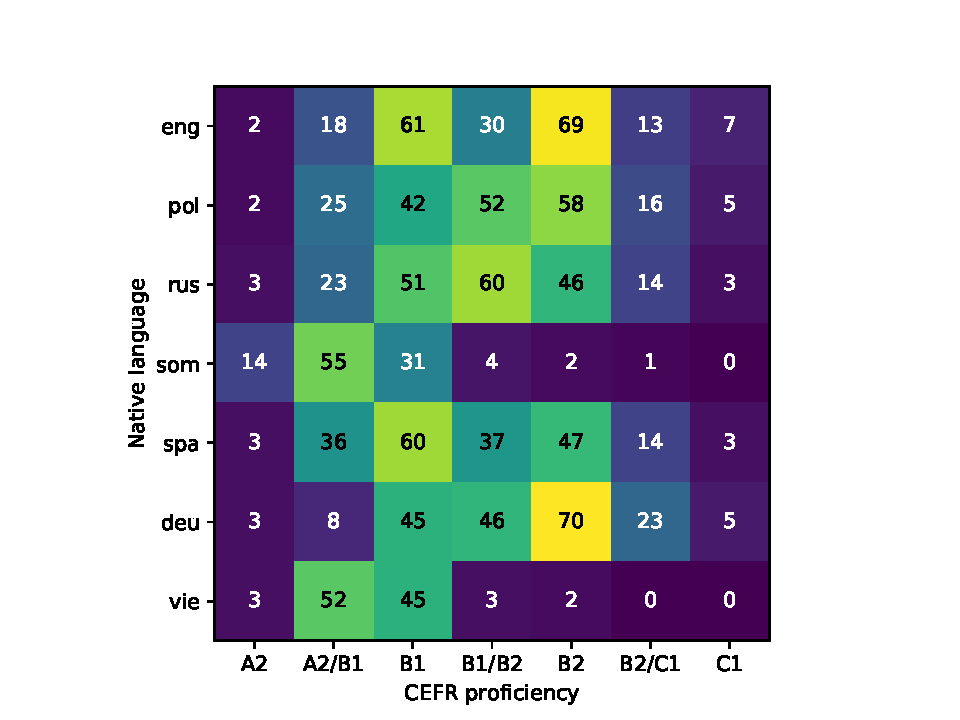
\includegraphics{lang_vs_cefr}
  \caption{The distribution of proficiency scores for each L1}
  \label{fig:lang-vs-cefr}
\end{figure}
 
\begin{figure}
  \centering
  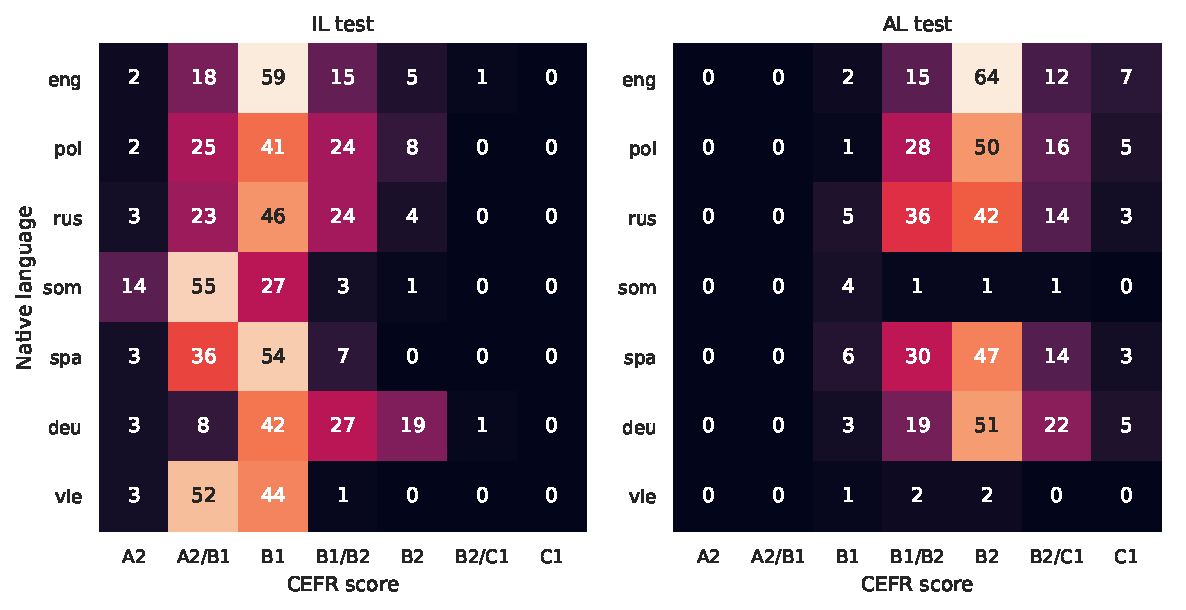
\includegraphics{testlevel_lang_vs_cefr}
  \caption{L1 versus CEFR score for each test level}
  \label{fig:testlevel-lang-vs-cefr}
\end{figure}

We analyze the data set in order to find correlations between different
metadata. Knowing that the documents stem from two different language tests
that measure different levels of proficiency, the data set was split in two
using the \emph{Test level} label, and then broken down by language and
proficiency again. Figure \ref{fig:testlevel-lang-vs-cefr} shows that the
test levels have different distributions of proficiency. Note also that two
language groups are underrepresented at the B2 test level (\emph{AL test}),
namely Somali and Vietnamese, which have seven and five essays in the B2 test
level, respectively. All other combinations of L1 and test level contain
exactly 100 essays. This partly explains the low average proficiency of
Somali and Vietnamese speakers apparent in figure \ref{fig:lang-vs-cefr}. The
difference compared to the other language groups is not as salient when
looking only at the B1 test level (\emph{IL test}) data.

\begin{table}
  \centering
  \begin{tabular}{lrrr}
    \toprule
    Topic                    & AL test & IL test & Total \\
    \midrule
    % cspell:disable
    telefon                  &      37 &      64 &   101 \\
    bolig                    &       0 &      83 &    83 \\
    familie helse vekt       &      59 &       0 &    59 \\
    tid                      &       2 &      51 &    53 \\
    natur norge              &       0 &      48 &    48 \\
    folk relasjoner vennskap &       0 &      45 &    45 \\
    tradisjoner flytting     &       0 &      38 &    38 \\
    barn                     &       3 &      32 &    35 \\
    kultur norge             &       0 &      34 &    34 \\
    media                    &       0 &      31 &    31 \\
    % cspell:enable
    \bottomrule
  \end{tabular}
  \caption[Most common topics in ASK texts]{
    The number of texts in each test level for the top 10 topics
    across test level.
  }
  \label{tab:texts-per-topic}
\end{table}

Another interesting variable is the essay topic. There is generally a strong
correlation between topic and vocabulary, and not accounting for this may
lead to a model picking up the wrong signal. Since the data is collected from
two different language tests, we might expect the distribution of topics to
differ between the test levels, and this is the case. Looking at the ten most
common topics in the data (table \ref{tab:texts-per-topic}), several are only
present on one test level.

There is also a difference in granularity. There are 52 topics in ``Høyere
nivå'' and only 38 topics in \emph{IL test}, even though there are more
documents in the latter test level (512 vs. 700). This also means that the
topics within each test level have different support. The median number of
documents for a topic in \emph{AL test} is 5 (mean $9.8$), while it is 11 in
\emph{IL test} (mean $18.4$). This also explains the overrepresentation of
\emph{IL test} in the table of top ten topics.

% cspell:disable
It has been observed that some topics in the diagram consist of several
sub-topics (for instance, ``natur norge'' consists of ``natur'' and
``norge''). However, the number of individual sub-topics is 62, still quite
large. However, they seem to be more evenly distributed across essays. The
median number of documents for a sub-topic, for both test levels, is 25 (mean
$34.8$). 13 sub-topics are only represented in 5 or fewer documents.
% cspell:enable

\begin{figure}
  \centering
  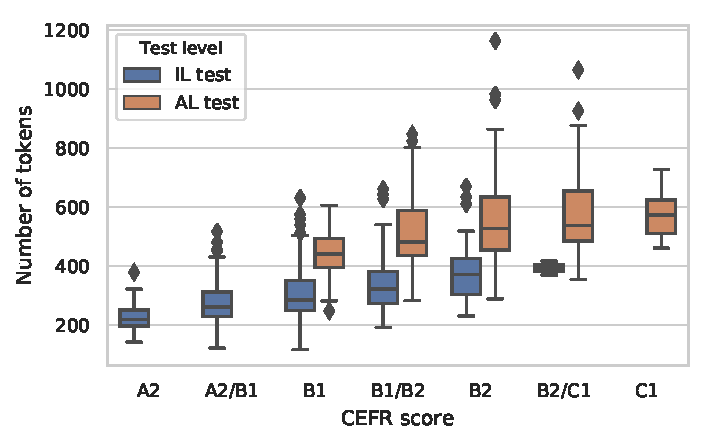
\includegraphics{testlevel_lengths_per_cefr}
  \caption[Document lengths on each CEFR level]{
    Distributions of essay lengths for CEFR scores on each test level.
  }
  \label{fig:testlevel-lengths-per-cefr}
\end{figure}

Document lengths have been seen to correlate with essay score in other
studies such as \textcite{vajjala17}. To see the relationship between these
variables in ASK, we again break down the data into the two test levels. One
group, \emph{B2/C1} CEFR score within \emph{IL test}, was excluded due to
having fewer than ten documents. Looking at figure
\ref{fig:testlevel-lengths-per-cefr}, two relations are apparent. Essays in
the \emph{AL test} test level are generally longer than in \emph{IL test},
and within each test level the higher scoring essays are generally longer.
Also, outliers are generally on the long side.

Note that even for the same CEFR score, the essays from the higher test level
are considerably longer. As an example, consider the \emph{B1/B2} score,
which is the most evenly distributed between the two test levels (101 essays
in \emph{IL test}, 131 in \emph{AL test}). More than 75\% of these texts on
the lower test level have fewer than 400 tokens, and more than 75\% on the
higher level are longer than 400 tokens. In fact, for all four CEFR scores
that are present on both test levels, there is no overlap of the
interquartile ranges\footnote{The range of values when the top 25\% and
bottom 25\% are excluded} between IL and AL test level.


\section{Data split}

At the start of the project, the dataset was split into a training,
development and test set in a 8:1:1 proportion. Ideally, the train and test
sets would have the same distribution of classes, but the limited amount of
data made this more difficult. As can be seen from figure
\ref{fig:lang-vs-cefr}, 15 of the combinations language vs. proficiency label
consist of only three or fewer documents.

Moreover, we wanted each split to consist of text topics not present in the
other splits. The reason for this to prevent a model from learning a bias for
topic. Finding a split that satisfies our constraints is an optimization
problem for which it can be intractable to find an optimal solution. We
therefore turned to heuristics, hoping that it would help us find a good
local optimum.
 
The split was chosen in order to have the right proportion of documents in
each part of the split, and so the distribution of proficiency and native
language is as similar as possible across the separate parts of the data
split. Specifically, the split was found by running an evolutionary algorithm
with a fitness function favouring splits that were as close as possible to
8:1:1 in proportion, while ensuring that each split contained a disjoint set
of topics.

We designed a fitness function incurred several penalties. A candidate split
was given a size penalty proportional to the absolute difference between the
sizes of test and dev splits and the wanted size, namely 10\% of the corpus.
Further, we added a label distribution penalty by calculating the
Kullback-Leibler divergences between the distributions of CEFR and L1 labels
in the candidate splits and the distribution in the entire corpus.
Kullback-Leibler divergence was computed using the SciPy \autocite{scipy}
library. The divergence values were squared and added to the penalty.

\begin{table}
  \centering
  \begin{tabular}{ll}
    \toprule
    Topics in development set &       Topics in test set \\
    \midrule
    % cspell:disable
         idrett/sport kultur &       geografi norge folk \\
                organisasjon &               innvandring \\
                  opplevelse & innvandring politikk valg \\
                     økonomi &              idrett/sport \\
                    holdning &            bolig geografi \\
           barn idrett/sport &               arbeid yrke \\
            familie flytting &          økonomi holdning \\
               eldre familie &              humor kultur \\
               helse røyking &   politikk norge holdning \\
       litteratur dikt språk &            litteratur bok \\
    helse arbeid innvandring &  familie befolkning norge \\
                barn familie &    litteratur dikt idrett \\
                       helse &           folk utdannelse \\
            utdannelse språk &         politikk holdning \\
          arbeid innvandring &                  media tv \\
      litteratur dikt venner &                  religion \\
                             &               helse organ \\
                             &             folk følelser \\
    % cspell:enable
    \bottomrule
  \end{tabular}
  \caption[Essay topics in development and test sets]{
    The topics chosen to be in each of the development and test sets.
  }
  \label{tab:topics-in-split}
\end{table}

% cspell:disable
The split in terms of the topics can be seen in table
\ref{tab:topics-in-split} \footnote{In the XML files, the topic values
contain a trailing space character, not visible in print.}. The dev and test
sets contain 123 texts each, close to the ideal 10\% of the corpus, which is
121. The topic variable has values which are sets of keywords, and therefore
there is still topical overlap between splits. For example, `økonomi'
(economy) and `økonomi holdning' (economy attitude) are considered separate
values and assigned to different splits, even though both topics include the
`economy' keyword.
% cspell:enable

\begin{figure}
  \centering
  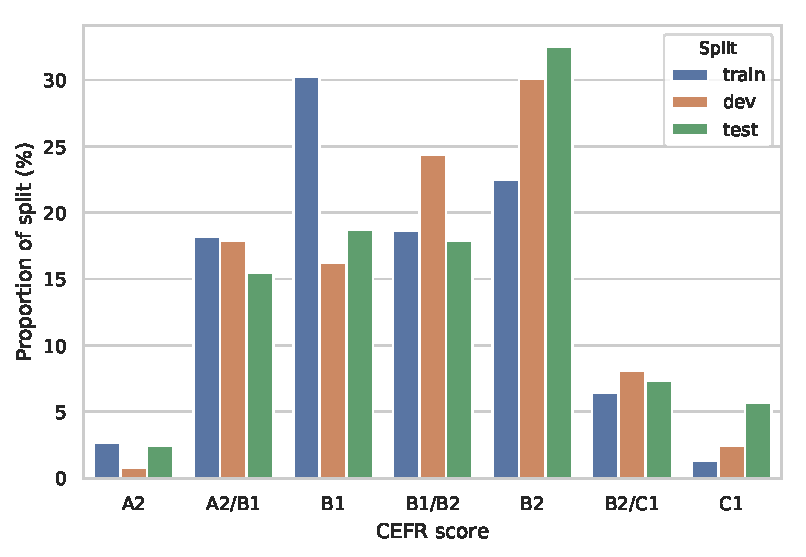
\includegraphics[width=\textwidth]{split-cefr-dist}
  \caption{Proportional distribution of CEFR labels in the three splits.}
  \label{fig:split-cefr-dist}
\end{figure}

\begin{figure}
  \centering
  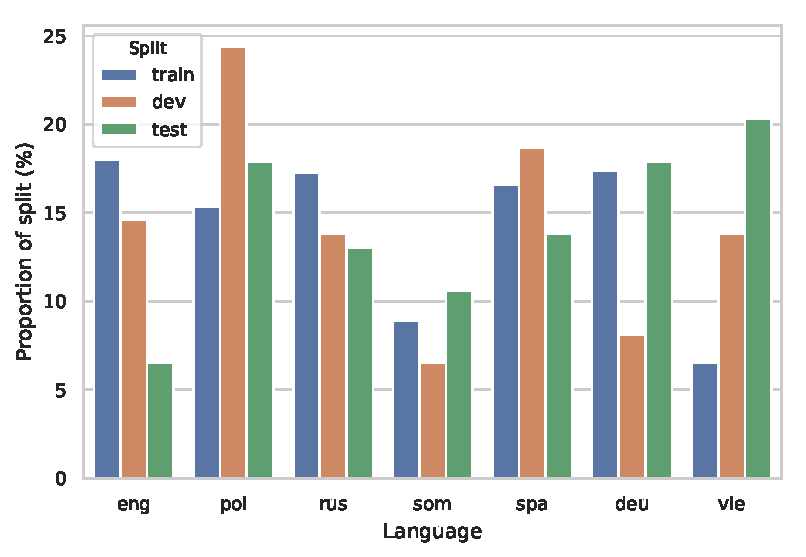
\includegraphics[width=\textwidth]{split-lang-dist}
  \caption{Proportional distribution of language labels in the three splits.}
  \label{fig:split-lang-dist}
\end{figure}

Figure \ref{fig:split-cefr-dist} shows how CEFR labels are distributed in the
resulting training, development and test splits, and figure
\ref{fig:split-lang-dist} shows the same for language labels. It can be seen
that all splits contain texts on all CEFR levels and for all different
\acp{L1}. While there are considerable differences in the distributions, we
decided that the result was reasonable given the constraints and the small
size of the dataset.

Each split does not contain every combination of CEFR score and \ac{L1}. This
follows from the distribution plotted in figure \ref{fig:lang-vs-cefr}, where
we find five combinations of CEFR score and \ac{L1} that occur only once or
twice. Since each document is assigned to exactly one of three different
splits, these combinations must necessarily be absent from one or two of the
splits.


\chapter{Experiments}


\section{Preprocessing}

The data files in the ASK corpus are in XML format, and contain information
about tags, mistakes and corrections, paragraphs, sentences and more. These
files were transformed into other formats during the process. First, they
were converted to plain text files stripped of all tags or correction labels,
with one sentence per line consisting of space-separated tokens, and an empty
line separating paragraphs.

These raw text files were then sent through the UDPipe pipeline for tagging
and dependency parsing. The output from UDPipe is in the CoNLL file format
with a single token per line. UDPipe tags the documents using the UD tagset,
while the original tags in the XML documents are from the Oslo-Bergen
tagger's own tagset.

\section{Baseline}

A logistic regression classifier was able to predict the CEFR score with
43.9\% accuracy using only two features: The length of the document, in
number of tokens, and the test level (IL test or AL test). 54 of 123
documents in the dev set.

A convolutional neural network based on the architecture in
\textcite{zhang2017sensitivity} achieved an accuracy of 42.3\% using
sequences of POS tags as input to an initial embedding layer.

Note that always predicting the majority class in the dev set (B2 with 37
documents) yields an accuracy of 30.1\%.


\backmatter{}

\printbibliography

\end{document}
